\documentclass[a4paper,12pt]{article}
\usepackage[top=1in, bottom=1in, left=1in, right=1in]{geometry}
\usepackage{amsmath, amssymb}
\usepackage{graphicx}
\usepackage{hyperref}
\usepackage{float}

\title{Orbiting Bodies: Analysis and Observations}
\author{Syed Arham Naqvi \\ 100590852}
\date{\today}

\begin{document}

\maketitle

\section{Introduction}
In this report, we discuss the modifications implemented to achieve a stable orbit in our simulation.

\section{Discussion}
The velocity of an object in stable orbit depends on the centripetal force on that object. In our simulation, the centripetal force on the moon allowing it to orbit the earth
is the force of gravity exerted on the moon by the earth. Using this model and the definition of centripetal force, we can derive the orbiting velocity required for the moon to maintain
a stable orbit given its mass, the earth's mass, its distance to the earth as well as the gravitational constant:

\begin{align*}
    F_{c}                                 &= F_{g} \\
    \frac{m_{moon} \cdot v_{moon}^{2}}{R} &= \frac{G \cdot m_{earth} \cdot m_{moon}}{R^{2}} \\
    v_{moon}                              &= \sqrt{\frac{G \cdot m_{earth}}{R}} \\
\end{align*}

After calculating this value we see the simulation immediately becomes far more stable
and the moon no longer falls to the earth or flies off the screen.
\\
\\
Next, Euler's method is inherently inaccurate as it assumes constant velocity for the
duration of the step despite the existence of acceleration. Consequently, there is a
perpetual addition of energy into the system by way of increasing velocities along the
x and y components. We thus observe the moon slowly drifting away from the earth as
evident by a shifting sin wave in the final analysis.
To address this, we use the RK4 ODE solver from scipy to calculate more accurate updates
for the velocities and position values.

The centripetal force between the bodies is calculated before each update based on the
latest positions of the bodies. We can then use the components of the force vector to
derive the following differential equations:
\begin{align*}
    \text{Motion Along the x Axis:}\\
    \frac{dv_x}{dt} &= \frac{Fg_x}{m}\\
    \frac{dx}{dt}   &= v_x\\
\end{align*}
\begin{align*}
    \text{Motion Along the y Axis:}\\
    \frac{dv_y}{dt} &= \frac{Fg_y}{m}\\
    \frac{dy}{dt}   &= v_y\\
\end{align*}

After implementing the above steps we note the following charts reflecting strong
simulation stability:

\begin{figure}[H]
    \centering
    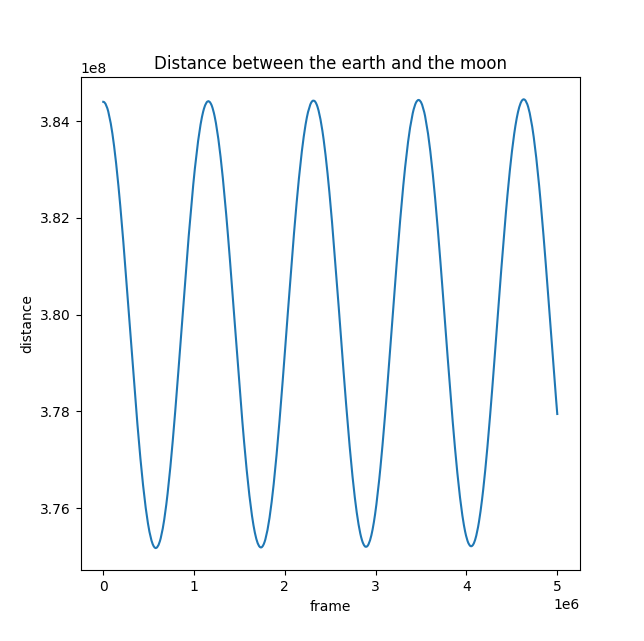
\includegraphics[width=0.8\textwidth]{./distances.png}
    \caption{Stable Distances Indicating Elliptical Orbit}
\end{figure}
\begin{figure}[H]
    \centering
    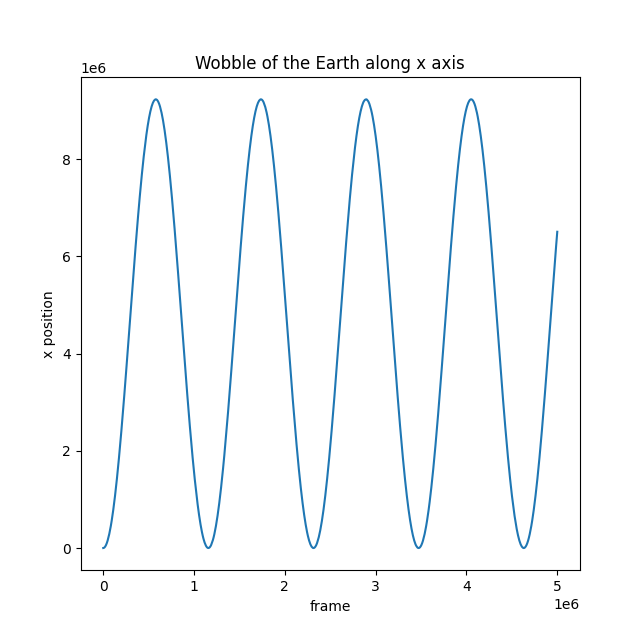
\includegraphics[width=0.8\textwidth]{./x_fluctuations.png}
    \caption{Wobble of the Earth Along x Axis}
\end{figure}

\end{document}
